%%
% Copyright (c) 2017 - 2024, Pascal Wagler;
% Copyright (c) 2014 - 2024, John MacFarlane
%
% All rights reserved.
%
% Redistribution and use in source and binary forms, with or without
% modification, are permitted provided that the following conditions
% are met:
%
% - Redistributions of source code must retain the above copyright
% notice, this list of conditions and the following disclaimer.
%
% - Redistributions in binary form must reproduce the above copyright
% notice, this list of conditions and the following disclaimer in the
% documentation and/or other materials provided with the distribution.
%
% - Neither the name of John MacFarlane nor the names of other
% contributors may be used to endorse or promote products derived
% from this software without specific prior written permission.
%
% THIS SOFTWARE IS PROVIDED BY THE COPYRIGHT HOLDERS AND CONTRIBUTORS
% "AS IS" AND ANY EXPRESS OR IMPLIED WARRANTIES, INCLUDING, BUT NOT
% LIMITED TO, THE IMPLIED WARRANTIES OF MERCHANTABILITY AND FITNESS
% FOR A PARTICULAR PURPOSE ARE DISCLAIMED. IN NO EVENT SHALL THE
% COPYRIGHT OWNER OR CONTRIBUTORS BE LIABLE FOR ANY DIRECT, INDIRECT,
% INCIDENTAL, SPECIAL, EXEMPLARY, OR CONSEQUENTIAL DAMAGES (INCLUDING,
% BUT NOT LIMITED TO, PROCUREMENT OF SUBSTITUTE GOODS OR SERVICES;
% LOSS OF USE, DATA, OR PROFITS; OR BUSINESS INTERRUPTION) HOWEVER
% CAUSED AND ON ANY THEORY OF LIABILITY, WHETHER IN CONTRACT, STRICT
% LIABILITY, OR TORT (INCLUDING NEGLIGENCE OR OTHERWISE) ARISING IN
% ANY WAY OUT OF THE USE OF THIS SOFTWARE, EVEN IF ADVISED OF THE
% POSSIBILITY OF SUCH DAMAGE.
%%

%%
% This is the Eisvogel pandoc LaTeX template.
%
% For usage information and examples visit the official GitHub page:
% https://github.com/Wandmalfarbe/pandoc-latex-template
%%

% Options for packages loaded elsewhere
\PassOptionsToPackage{unicode}{hyperref}
\PassOptionsToPackage{hyphens}{url}
\PassOptionsToPackage{dvipsnames,svgnames,x11names,table}{xcolor}
%
\documentclass[
  paper=a4,
  ,captions=tableheading
]{scrartcl}
\usepackage{amsmath,amssymb}
% Use setspace anyway because we change the default line spacing.
% The spacing is changed early to affect the titlepage and the TOC.
\usepackage{setspace}
\setstretch{1.2}
\usepackage{iftex}
\ifPDFTeX
  \usepackage[T1]{fontenc}
  \usepackage[utf8]{inputenc}
  \usepackage{textcomp} % provide euro and other symbols
\else % if luatex or xetex
  \usepackage{unicode-math} % this also loads fontspec
  \defaultfontfeatures{Scale=MatchLowercase}
  \defaultfontfeatures[\rmfamily]{Ligatures=TeX,Scale=1}
\fi
\usepackage{lmodern}
\ifPDFTeX\else
  % xetex/luatex font selection
\fi
% Use upquote if available, for straight quotes in verbatim environments
\IfFileExists{upquote.sty}{\usepackage{upquote}}{}
\IfFileExists{microtype.sty}{% use microtype if available
  \usepackage[]{microtype}
  \UseMicrotypeSet[protrusion]{basicmath} % disable protrusion for tt fonts
}{}
\makeatletter
\@ifundefined{KOMAClassName}{% if non-KOMA class
  \IfFileExists{parskip.sty}{%
    \usepackage{parskip}
  }{% else
    \setlength{\parindent}{0pt}
    \setlength{\parskip}{6pt plus 2pt minus 1pt}}
}{% if KOMA class
  \KOMAoptions{parskip=half}}
\makeatother
\usepackage{xcolor}
\definecolor{default-linkcolor}{HTML}{A50000}
\definecolor{default-filecolor}{HTML}{A50000}
\definecolor{default-citecolor}{HTML}{4077C0}
\definecolor{default-urlcolor}{HTML}{4077C0}
\usepackage[top=1.3in,bottom=1in,left=1in,right=1in]{geometry}
\usepackage[export]{adjustbox}
\usepackage{graphicx}
\usepackage{etoolbox}
\BeforeBeginEnvironment{lstlisting}{\par\noindent\begin{minipage}{\linewidth}}
\AfterEndEnvironment{lstlisting}{\end{minipage}\par\addvspace{\topskip}}
\usepackage{longtable,booktabs,array}
\usepackage{calc} % for calculating minipage widths
% Correct order of tables after \paragraph or \subparagraph
\usepackage{etoolbox}
\makeatletter
\patchcmd\longtable{\par}{\if@noskipsec\mbox{}\fi\par}{}{}
\makeatother
% Allow footnotes in longtable head/foot
\IfFileExists{footnotehyper.sty}{\usepackage{footnotehyper}}{\usepackage{footnote}}
\makesavenoteenv{longtable}
% add backlinks to footnote references, cf. https://tex.stackexchange.com/questions/302266/make-footnote-clickable-both-ways
\usepackage{footnotebackref}
\usepackage{graphicx}
\makeatletter
\newsavebox\pandoc@box
\newcommand*\pandocbounded[1]{% scales image to fit in text height/width
  \sbox\pandoc@box{#1}%
  \Gscale@div\@tempa{\textheight}{\dimexpr\ht\pandoc@box+\dp\pandoc@box\relax}%
  \Gscale@div\@tempb{\linewidth}{\wd\pandoc@box}%
  \ifdim\@tempb\p@<\@tempa\p@\let\@tempa\@tempb\fi% select the smaller of both
  \ifdim\@tempa\p@<\p@\scalebox{\@tempa}{\usebox\pandoc@box}%
  \else\usebox{\pandoc@box}%
  \fi%
}
% Set default figure placement to htbp
% Make use of float-package and set default placement for figures to H.
% The option H means 'PUT IT HERE' (as  opposed to the standard h option which means 'You may put it here if you like').
\usepackage{float}
\floatplacement{figure}{H}
\makeatother

%% change the default with of the images using \setkeys{Gin}{width=.8\linewidth}
\setkeys{Gin}{width=1\linewidth}
\setlength{\emergencystretch}{3em} % prevent overfull lines
\providecommand{\tightlist}{%
  \setlength{\itemsep}{0pt}\setlength{\parskip}{0pt}}
\setcounter{secnumdepth}{-\maxdimen} % remove section numbering
\ifLuaTeX
\usepackage[bidi=basic]{babel}
\else
\usepackage[bidi=default]{babel}
\fi
\babelprovide[main,import]{english}
% get rid of language-specific shorthands (see #6817):
\let\LanguageShortHands\languageshorthands
\def\languageshorthands#1{}
\makeatletter
\@ifpackageloaded{subfig}{}{\usepackage{subfig}}
\@ifpackageloaded{caption}{}{\usepackage{caption}}
\captionsetup[subfloat]{margin=0.5em}
\AtBeginDocument{%
\renewcommand*\figurename{Figura}
\renewcommand*\tablename{Tabla}
}
\AtBeginDocument{%
\renewcommand*\listfigurename{Lista de Figuras}
\renewcommand*\listtablename{Lista de Tablas}
}
\newcounter{pandoccrossref@subfigures@footnote@counter}
\newenvironment{pandoccrossrefsubfigures}{%
\setcounter{pandoccrossref@subfigures@footnote@counter}{0}
\begin{figure}\centering%
\gdef\global@pandoccrossref@subfigures@footnotes{}%
\DeclareRobustCommand{\footnote}[1]{\footnotemark%
\stepcounter{pandoccrossref@subfigures@footnote@counter}%
\ifx\global@pandoccrossref@subfigures@footnotes\empty%
\gdef\global@pandoccrossref@subfigures@footnotes{{##1}}%
\else%
\g@addto@macro\global@pandoccrossref@subfigures@footnotes{, {##1}}%
\fi}}%
{\end{figure}%
\addtocounter{footnote}{-\value{pandoccrossref@subfigures@footnote@counter}}
\@for\f:=\global@pandoccrossref@subfigures@footnotes\do{\stepcounter{footnote}\footnotetext{\f}}%
\gdef\global@pandoccrossref@subfigures@footnotes{}}
\@ifpackageloaded{float}{}{\usepackage{float}}
\floatstyle{ruled}
\@ifundefined{c@chapter}{\newfloat{codelisting}{h}{lop}}{\newfloat{codelisting}{h}{lop}[chapter]}
\floatname{codelisting}{Listing}
\newcommand*\listoflistings{\listof{codelisting}{Listas del Documento}}
\makeatother
\usepackage{bookmark}
\IfFileExists{xurl.sty}{\usepackage{xurl}}{} % add URL line breaks if available
\urlstyle{same}
\hypersetup{
  pdftitle={Propuesta de Servicios Banco Mundo Mujer},
  pdfauthor={SoftProductiva.com},
  pdflang={en},
  pdfsubject={Proyecto de Evaluación y Hoja de Ruta Arquitectura},
  pdfkeywords={Arquitectura, Evaluación, Diseño, Hoja de
ruta, Transición},
  hidelinks,
  breaklinks=true,
  pdfcreator={LaTeX via pandoc with the Eisvogel template}}
\title{Propuesta de Servicios Banco Mundo Mujer}
\usepackage{etoolbox}
\makeatletter
\providecommand{\subtitle}[1]{% add subtitle to \maketitle
  \apptocmd{\@title}{\par {\large #1 \par}}{}{}
}
\makeatother
\subtitle{Evaluación y Hoja de Ruta de la Arquitectura del Canal
Bancario Whatsapp}
\author{SoftProductiva.com}
\date{2025-01-20}



%%
%% added
%%


%
% for the background color of the title page
%
\usepackage{pagecolor}
\usepackage{afterpage}
\usepackage{tikz}

%
% break urls
%
\PassOptionsToPackage{hyphens}{url}

%
% When using babel or polyglossia with biblatex, loading csquotes is recommended
% to ensure that quoted texts are typeset according to the rules of your main language.
%
\usepackage{csquotes}

%
% captions
%
\definecolor{caption-color}{HTML}{777777}
\usepackage[font={stretch=1.2}, textfont={color=caption-color}, position=top, skip=4mm, labelfont=bf, singlelinecheck=false, justification=raggedright]{caption}
\setcapindent{0em}

%
% blockquote
%
\definecolor{blockquote-border}{RGB}{221,221,221}
\definecolor{blockquote-text}{RGB}{119,119,119}
\usepackage{mdframed}
\newmdenv[rightline=false,bottomline=false,topline=false,linewidth=3pt,linecolor=blockquote-border,skipabove=\parskip]{customblockquote}
\renewenvironment{quote}{\begin{customblockquote}\list{}{\rightmargin=0em\leftmargin=0em}%
\item\relax\color{blockquote-text}\ignorespaces}{\unskip\unskip\endlist\end{customblockquote}}

%
% Source Sans Pro as the default font family
% Source Code Pro for monospace text
%
% 'default' option sets the default
% font family to Source Sans Pro, not \sfdefault.
%
\ifnum 0\ifxetex 1\fi\ifluatex 1\fi=0 % if pdftex
    \usepackage[default]{sourcesanspro}
  \usepackage{sourcecodepro}
  \else % if not pdftex
    \usepackage[default]{sourcesanspro}
  \usepackage{sourcecodepro}

  % XeLaTeX specific adjustments for straight quotes: https://tex.stackexchange.com/a/354887
  % This issue is already fixed (see https://github.com/silkeh/latex-sourcecodepro/pull/5) but the
  % fix is still unreleased.
  % TODO: Remove this workaround when the new version of sourcecodepro is released on CTAN.
  \ifxetex
    \makeatletter
    \defaultfontfeatures[\ttfamily]
      { Numbers   = \sourcecodepro@figurestyle,
        Scale     = \SourceCodePro@scale,
        Extension = .otf }
    \setmonofont
      [ UprightFont    = *-\sourcecodepro@regstyle,
        ItalicFont     = *-\sourcecodepro@regstyle It,
        BoldFont       = *-\sourcecodepro@boldstyle,
        BoldItalicFont = *-\sourcecodepro@boldstyle It ]
      {SourceCodePro}
    \makeatother
  \fi
  \fi

%
% heading color
%
\definecolor{heading-color}{RGB}{40,40,40}
\addtokomafont{section}{\color{heading-color}}
% When using the classes report, scrreprt, book,
% scrbook or memoir, uncomment the following line.
%\addtokomafont{chapter}{\color{heading-color}}

%
% variables for title, author and date
%
\usepackage{titling}
\title{Propuesta de Servicios Banco Mundo Mujer}
\author{SoftProductiva.com}
\date{2025-01-20}

%
% tables
%

\definecolor{table-row-color}{HTML}{F5F5F5}
\definecolor{table-rule-color}{HTML}{999999}

%\arrayrulecolor{black!40}
\arrayrulecolor{table-rule-color}     % color of \toprule, \midrule, \bottomrule
\setlength\heavyrulewidth{0.3ex}      % thickness of \toprule, \bottomrule
\renewcommand{\arraystretch}{0.8}     % spacing (padding)


%
% remove paragraph indentation
%
\setlength{\parindent}{0pt}
\setlength{\parskip}{6pt plus 2pt minus 1pt}
\setlength{\emergencystretch}{3em}  % prevent overfull lines

%
%
% Listings
%
%


%
% header and footer
%
\usepackage[headsepline,footsepline]{scrlayer-scrpage}

\newpairofpagestyles{eisvogel-header-footer}{
  \clearpairofpagestyles
  \ihead*{2025-01-20}
  \chead*{}
  \ohead*{Propuesta de Servicios Banco Mundo Mujer}
  \ifoot*{SoftProductiva.com}
  \cfoot*{}
  \ofoot*{\thepage}
  \addtokomafont{pageheadfoot}{\upshape}
}
\pagestyle{eisvogel-header-footer}



%%
%% end added
%%

\begin{document}

%%
%% begin titlepage
%%
\begin{titlepage}
\newgeometry{top=2cm, right=4cm, bottom=3cm, left=4cm}
\tikz[remember picture,overlay] \node[inner sep=0pt] at (current page.center){
\includegraphics[width=\paperwidth,height=\paperheight]{include/background2.pdf}};
\newcommand{\colorRule}[3][black]{\textcolor[HTML]{#1}{\rule{#2}{#3}}}
\begin{flushleft}
\noindent
\\[-1em]
\color[HTML]{5F5F5F}
\makebox[0pt][l]{\colorRule[360049]{1.3\textwidth}{4pt}}
\par
\noindent

% The titlepage with a background image has other text spacing and text size
{
  \setstretch{2}
  \vfill
  \vskip -8em
  \noindent {\huge \textbf{\textsf{Propuesta de Servicios Banco Mundo
Mujer}}}
    \vskip 1em
  {\Large \textsf{Evaluación y Hoja de Ruta de la Arquitectura del Canal
Bancario Whatsapp}}
    \vskip 2em
  \noindent {\Large \textsf{SoftProductiva.com} \vskip 0.6em \textsf{2025-01-20}}
  \vfill
}

\noindent

\includegraphics[width=60mm, right]{include/logo.png}


\end{flushleft}
\end{titlepage}
\restoregeometry
\pagenumbering{arabic}

%%
%% end titlepage
%%

% \maketitle


\newpage

\section{Información del
Documento}\label{sec:informaciuxf3n-del-documento}

Esta es la doc del grupo.

\subsection{Versión del Documento}\label{sec:versiuxf3n-del-documento}

\begin{quote}
\end{quote}

\subsection{Control de Cambios}\label{sec:control-de-cambios}

Historia de cambios de la propuesta.

Versión actual: 1.1ee976b - pdfyml - Mon, 17 Mar 2025 06:03:02 -0500

Versiones Anteriores

1.1b82157 - pdfyml - Mon, 17 Mar 2025 05:58:14 -0500

1.54a0299 - accion - Mon, 17 Mar 2025 05:33:46 -0500

1.025ce99 - contd/ruta - Sat, 8 Mar 2025 00:22:40 -0500

1.3a8fbed - titulo - Fri, 14 Feb 2025 13:17:17 -0500

\subsubsection{Realizado Por}\label{sec:realizado-por}

H. Wong, ing.

\subsubsection{Revisado Por}\label{sec:revisado-por}

(revisor), Canal Bancario Whatsapp

El Miedo a la Política (Superar) A. Laje (2024). Globalismo. (Extracto.
Pág. 551)

\newpage

\section{Servicios de Ingeniería Canal Bancario Whatsapp Banco Mundial
de la
Mujer}\label{sec:servicios-de-ingenieruxeda-canal-bancario-whatsapp-banco-mundial-de-la-mujer}

\subsection{Descripción de la
Propuesta}\label{sec:descripciuxf3n-de-la-propuesta}

\begin{quote}
\end{quote}

Consultoría de ingeniería y mejoramiento del canal bancario textual
Whatsapp del Banco Mundo Mujer (BMM), con extensión a sistemas externos,
legados y proveedores tecnológicos relacionados con la arquitectura del
canal.

\subsection{Detalles Técnicos de la
Propuesta}\label{sec:detalles-tuxe9cnicos-de-la-propuesta}

\begin{quote}
\end{quote}

Esta propuesta contienen los siguientes componentes técnicos.

\begin{itemize}
\tightlist
\item
  Metas del proyecto
\item
  Alcance
\item
  Métodos
\item
  Entregables
\item
  Plan de trabajo
\item
  Propuesta económica
\item
  Consideraciones y restricciones
\end{itemize}

\subsection{Metas de la Propuesta}\label{sec:metas-de-la-propuesta}

\begin{quote}
\end{quote}

\begin{enumerate}
\def\labelenumi{\arabic{enumi}.}
\tightlist
\item
  \textbf{Diagnóstico}. Hallazgos relevantes de la arquitectura del
  Canal Bancario Whatsapp. Presentar puntos de cambios relevantes
  resultado del análisis de la arquitectura de solución actual del canal
  de banca Whatsapp (chat) del Banco Mundial de la Mujer categorizados
  en varias perspectivas, como la funcional, técnica y operativa.
\item
  \textbf{Hoja de Ruta}. Lista de cambios y gestión de cambios de la de
  la arquitectura del Canal Bancario Whatsapp**. Desarrollar la hoja de
  ruta de los cambios derivados del objetivo no. 1, Hallazgos relevantes
  de la arquitectura, con una priorización planteada mediante criterio
  críticos de factibilidad e impacto a Banco Mundial de la Mujer.
\end{enumerate}

\subsection{Alcance}\label{sec:alcance}

\begin{quote}
\end{quote}

\begin{enumerate}
\def\labelenumi{\arabic{enumi}.}
\tightlist
\item
  Diagnóstico. Evaluación de la arquitectura del Canal Bancario Whatsapp
  del Banco Mundial de la Mujer que resulta en puntos de cambios
  accionables de la arquitectura del Canal Bancario Whatsapp.
\item
  Diseño de hoja de ruta de transformación. Planteamiento de transición
  de la arquitectura del Canal Bancario Whatsapp mediante lista de
  cambios priorizados sobre la arquitectura del canal.
\end{enumerate}

\subsubsection{Exclusiones del
Alcance}\label{sec:exclusiones-del-alcance}

La presenta propuesta no incluye:

\begin{enumerate}
\def\labelenumi{\arabic{enumi}.}
\tightlist
\item
  Por restricciones de tiempo, la actual propuesta no incluye análisis
  ni recomendaciones de diseño a arquitectura distintas a las del Canal
  Bancario Whatsapp.
\item
  No incluye plan de capacidad ni proyección de uso infraestructura
  futura de la arquitectura del Canal Bancario Whatsapp.
\item
  No incluye la provisión de infraestructura para las soluciones
  derivadas de este proyecto.
\item
  No incluye soporte ni mantenimiento posterior a la realización de este
  proyecto.
\end{enumerate}

\subsection{Método Propuesto}\label{sec:muxe9todo-propuesto}

\begin{quote}
\end{quote}

\begin{enumerate}
\def\labelenumi{\arabic{enumi}.}
\tightlist
\item
  Planificación. Período inicial de definición y acuerdos de los
  objetivos puntuales de las evaluación de la arquitectura del Canal
  Bancario Whatsapp.
\item
  Preparación y Alistamiento. Lista de chequeo de recursos, personas y
  procesos relacionadas con las vistas de arquitectura del Canal
  Bancario Whatsapp, como las vistas funcional, técnica, despliegues, y
  otras.
\item
  Definición. Confirmación del diseño de los escenarios de evaluación de
  la arquitectura del Canal Bancario Whatsapp. Identificación de otras
  dependencias entre escenarios.
\item
  Diagnóstico. Profundización del detalle de la información, ejecución
  de los métodos seleccionados para la evaluación de la arquitectura, y
  documentación reproducible de los resultados.
\item
  Verificación. Contrastar el resultado preliminar de los escenarios de
  evaluación de la arquitectura del Canal Bancario Whatsapp contra el
  método de evaluación.
\item
  Divulgación de Resultados y Entregables. (luego de la verificación)
  Explicar el resultado general de la evaluación de los escenarios de la
  arquitectura del Canal Bancario Whatsapp y discrepancias con umbrales
  de aceptación.
\item
  Diseño de Hoja de Ruta. Preparación, alistamiento y priorización de
  las transiciones de la arquitectura del Canal Bancario Whatsapp (hoja
  de ruta).
\item
  Divulgación de Resultados y Entregables Finales. Compilación de
  artefactos, documentación técnica y divulgación de conocimiento del
  resultado de diagnóstico y de la hoja de ruta priorizada de la
  arquitectura del Canal Bancario Whatsapp.
\end{enumerate}

\begin{figure}
\centering
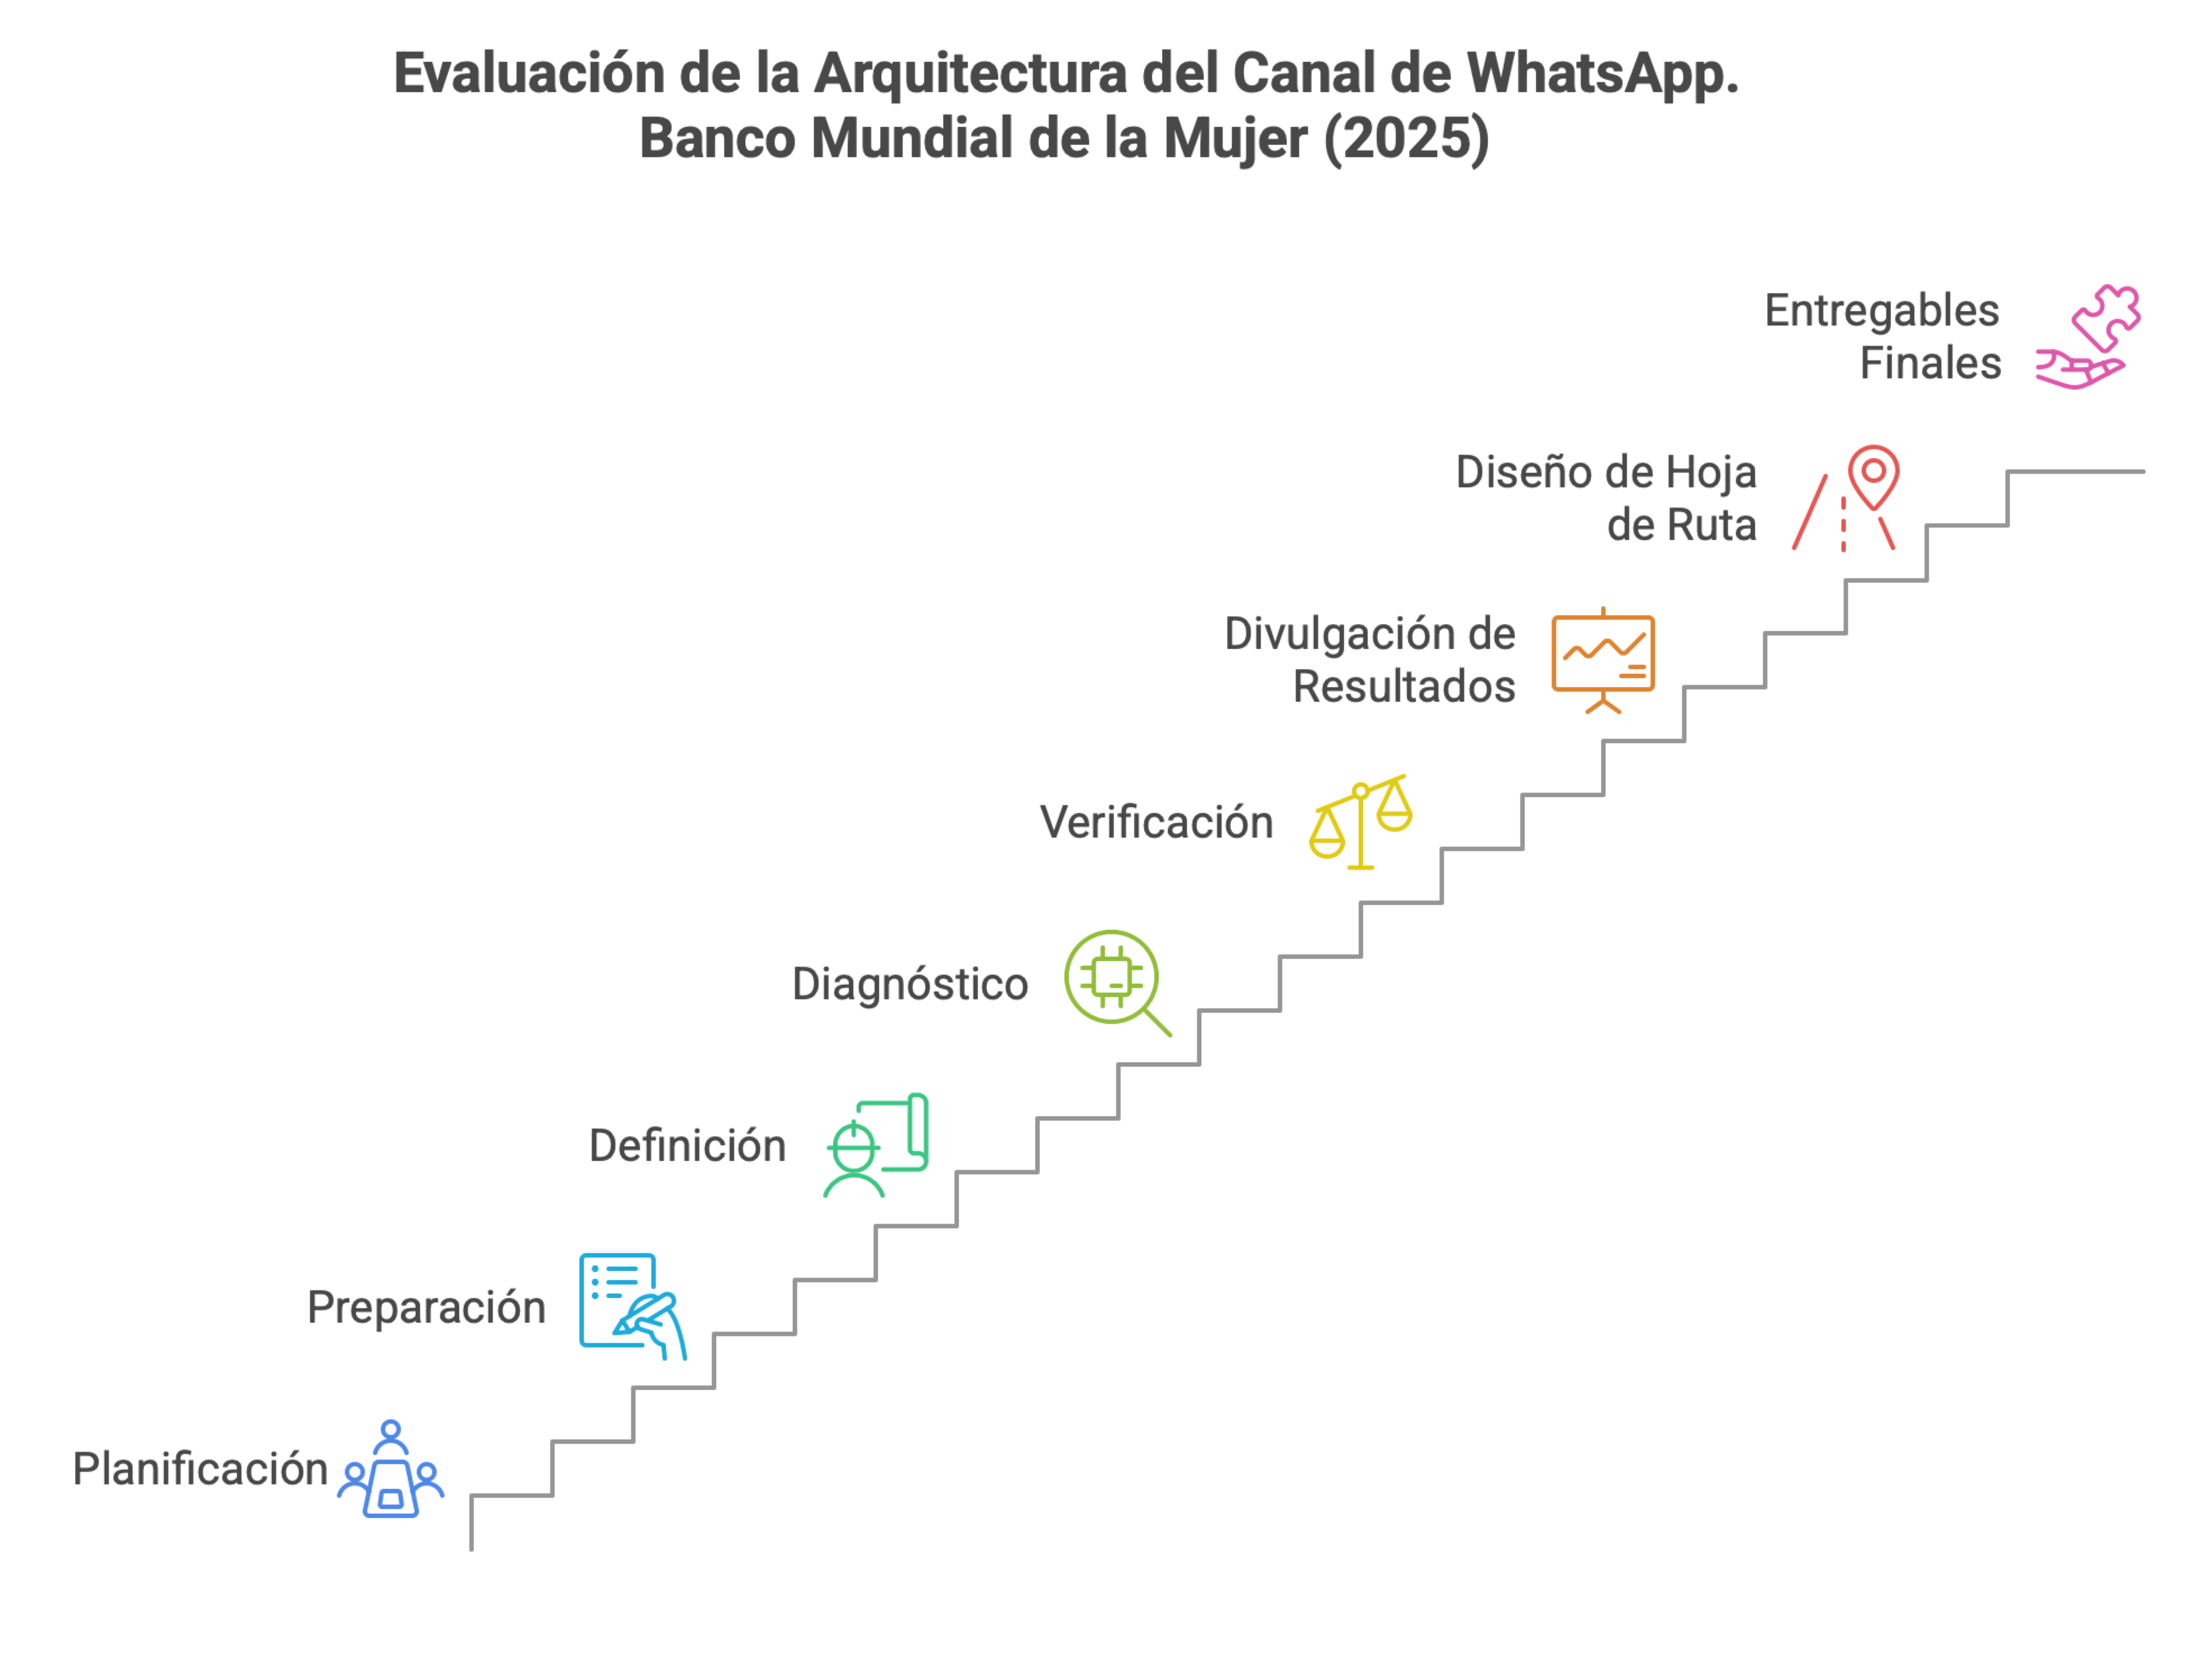
\includegraphics{images/02.1c.Metodo.png}
\caption{02.1c.Metodo. \emph{Fuente: Propuesta servicios de ingeniería y
evaluación de arquitectura Canal Bancario Whatsapp Banco Mundial de la
Mujer (2025)}}\label{fig:id-ecb3efe1a4e14dd389ece75370f1861c}
\end{figure}

\subsection{Entregables de la
Propuesta}\label{sec:entregables-de-la-propuesta}

\begin{quote}
\end{quote}

\begin{enumerate}
\def\labelenumi{\arabic{enumi}.}
\tightlist
\item
  Evaluación de la arquitectura del Canal Bancario Whatsapp del Banco
  Mundial de la Mujer. Listado de hallazgos relevantes y accionables de
  la arquitectura desde las perspectivas rendimiento, funcional-negocio,
  y operativa (esta perspectiva incluye a los métodos de construcción,
  pruebas y transición).
\item
  Hoja de ruta de las cambios requeridos y transformaciones para el
  mejoramiento de la arquitectura de Canal Bancario Whatsapp.
  Instrumento para la gestieon de cambios priorizados y planeación de la
  entrega de las transición de la arquitectura de Canal Bancario
  Whatsapp del Banco Mundial de la Mujer.
\end{enumerate}

\newpage

\section{Aspectos Técnicos de la
Propuesta}\label{sec:aspectos-tuxe9cnicos-de-la-propuesta}

\subsection{Plan de Trabajo}\label{sec:plan-de-trabajo}

\begin{quote}
\end{quote}

El plan de trabajo propuesto consta de dos fases consecutivas que
inician a partir de la aceptación y formalización de la actual
propuesta. La Fase I, llamada en esta propuesta el diagnóstico y
evaluación de la arquitectura; y la Fase II, destinada al diseño de la
hoja de ruta de transformación de la arquitectura del Canal Bancario
Whatsapp.

En detalle cada fase del proyecto:

\begin{enumerate}
\def\labelenumi{\arabic{enumi}.}
\item
  Día 1 al 15. Diagnóstico y evaluación de la arquitectura del Canal
  Bancario Whatsapp, incluye planificación, preparación, diagnóstico,
  documentación técnica, y divulgación: estimada en 15 días de trabajo.
\item
  Día 16 al 20. Diseño de hoja de ruta de transformación de la
  arquitectura del Canal Bancario Whatsapp, incluye diseño de hoja de
  ruta, ejecución transiciones, gestión de cambios, documentación
  técnica, divulgación: estimada en 5 días de trabajo.
\end{enumerate}

\subsection{Plazo de Ejecución}\label{sec:plazo-de-ejecuciuxf3n}

Por lo anterior, el total de la duración del proyecto es de un (1) mes
laboral.

\begin{figure}
\centering
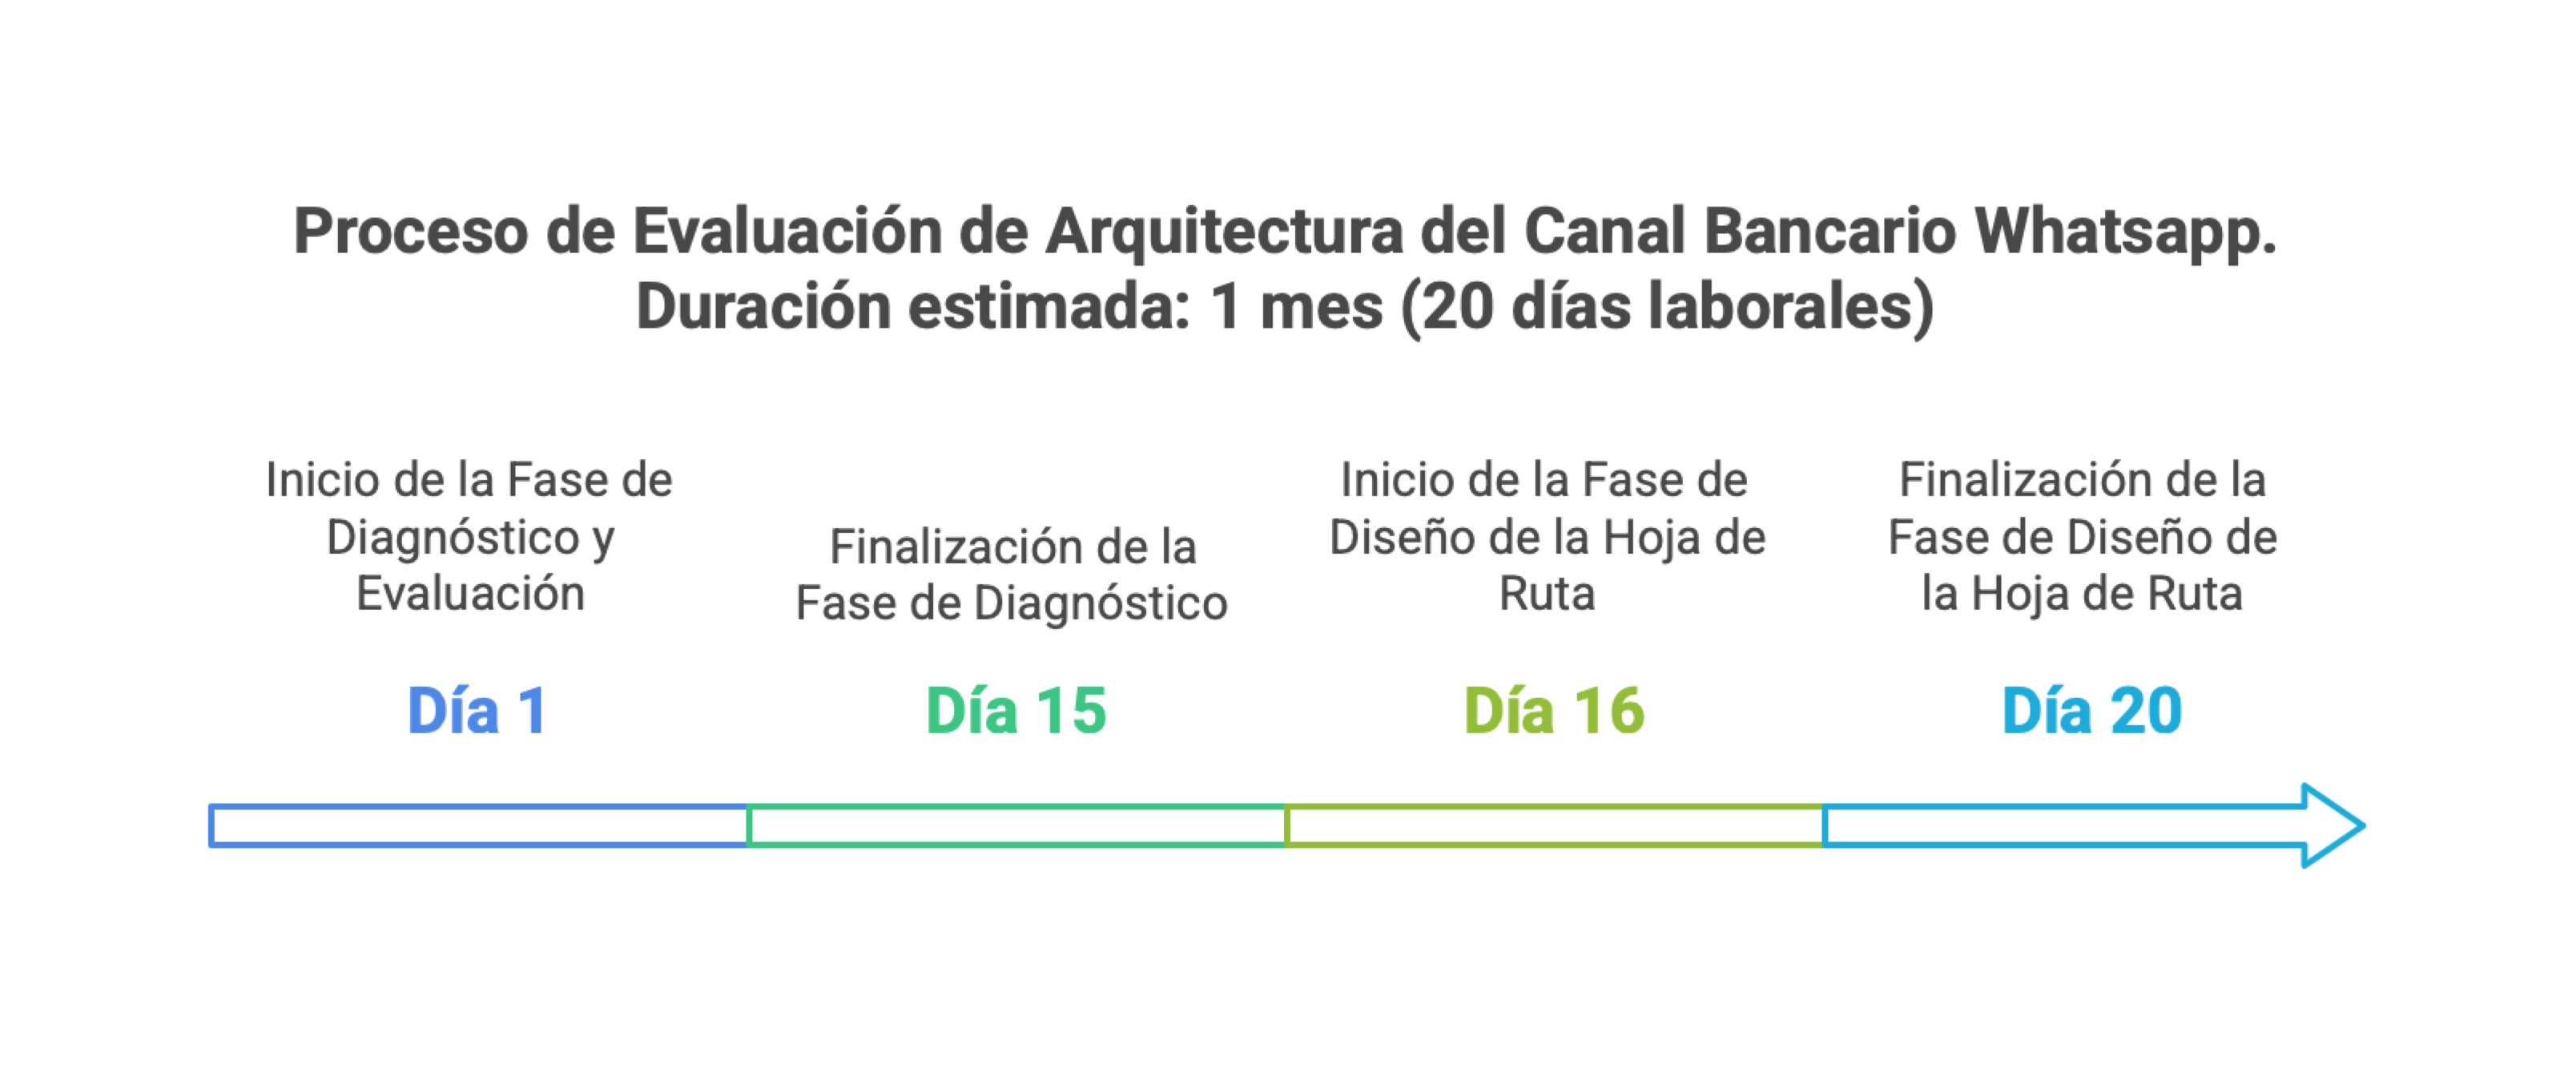
\includegraphics{images/02.1e1.Plan.png}
\caption{02.1e1.Plan. \emph{Fuente: Propuesta servicios de ingeniería y
evaluación de arquitectura Canal Bancario Whatsapp Banco Mundial de la
Mujer (2025)}}\label{fig:id-650dca2ba0114dca99ad6302b8ed6dc7}
\end{figure}

\subsection{Propuesta Económica}\label{sec:propuesta-econuxf3mica}

\begin{quote}
\end{quote}

A la presente propuesta, en los términos consignados aquí, le
corresponde la siguiente propuesta económica.

\begin{longtable}[]{@{}
  >{\raggedright\arraybackslash}p{(\columnwidth - 6\tabcolsep) * \real{0.5161}}
  >{\raggedright\arraybackslash}p{(\columnwidth - 6\tabcolsep) * \real{0.1828}}
  >{\raggedright\arraybackslash}p{(\columnwidth - 6\tabcolsep) * \real{0.1505}}
  >{\raggedright\arraybackslash}p{(\columnwidth - 6\tabcolsep) * \real{0.1505}}@{}}
\toprule\noalign{}
\begin{minipage}[b]{\linewidth}\raggedright
Ítem
\end{minipage} & \begin{minipage}[b]{\linewidth}\raggedright
Valor (COP \$/.)
\end{minipage} & \begin{minipage}[b]{\linewidth}\raggedright
IVA (19\%)
\end{minipage} & \begin{minipage}[b]{\linewidth}\raggedright
Total
\end{minipage} \\
\midrule\noalign{}
\endhead
\bottomrule\noalign{}
\endlastfoot
Evaluación y hoja de ruta de arquitectura Canal Bancario Whatsapp & \$
62'000,000 & \$ 11'400.000 & \$ 71'400.000 \\
Descuento del 10\% Cliente Primera Vez & \$ 6.000.000 & \$ 1.140.000 &
\$ 7.140.000 \\
TOTAL & \$ 54.000.000 & \$ 10.260.000 & \$ 64.260.000 \\
\end{longtable}

Nota: los valores del costo de la propuesta se mantienen durante los
siguientes 10 días laborales luego de su presentación a los interesados.

\subsubsection{Forma de Pago de la
Propuesta}\label{sec:forma-de-pago-de-la-propuesta}

\begin{longtable}[]{@{}lll@{}}
\toprule\noalign{}
Pagos & Fracción & Hito del Plan \\
\midrule\noalign{}
\endhead
\bottomrule\noalign{}
\endlastfoot
Primer pago & 50\% & Evaluación de la arquitectura \\
Segundo pago & 50\% & Hoja de Ruta Priorizada \\
\end{longtable}

\subsection{Equipo de Trabajo}\label{sec:equipo-de-trabajo}

\begin{quote}
\end{quote}

El equipo de trabajo requerido para el cumplimiento del alcance, metas y
entregables de la actual propuesta será provisto por el proponente.

Por las restricciones de ejecución usuales en este tipo de proyectos es
requerido apoyo interno de la empresa cliente del Canal Bancario
Whatsapp.

El nivel de participación en el proyecto y el rol del recurso interno se
acuerdan a conveniencia de las partes, cliente y proponente.

\subsection{Consideraciones
Importantes}\label{sec:consideraciones-importantes}

\begin{quote}
\end{quote}

\begin{enumerate}
\def\labelenumi{\arabic{enumi}.}
\tightlist
\item
  Forma de pago de la propuesta: 50\% al final del primer entregables,
  50\% al final del segundo entregable.
\item
  Por las restricciones propias de proyecto la ejecución de este
  proyecto requiere apoyo de un ingeniero interno de la empresa,
  dedicado el tiempo convenido entre las partes.
\item
  Las estimaciones de costo, esfuerzo, tiempo, y planeación son
  aproximadas, y representan la intención de la propuesta basada en la
  información conocida por las partes al momento de su realización.
\item
  Las extensiones en los entregables, o cambios a la propuesta se
  acordarán en definiciones y extensiones por separado.
\end{enumerate}

\newpage

\section{Resumen de la Propuesta}\label{sec:resumen-de-la-propuesta}

\subsection{}\label{sec:section}

\begin{quote}
\end{quote}

\begin{itemize}
\tightlist
\item
  El resultado del proyecto es el diagnóstico y la lista de cambios
  priorizados sobre la arquitectura del Canal Bancario Whatsapp, la
  divulgación de los cambios y la documentación técnica
\item
  La duración del proyecto es de un (1) mes de trabajo (días laborales).
\item
  El equipo de trabajo propuesto será provisto por el proponente.
\item
  El valor económico de la propuesta es \$64.260.000 COP, IVA incluido.
\item
  Esta propuesta no incluye recomendaciones de diseño, intervenciones a
  sistemas distintos de los consignados en el alcance, ni servicios de
  infraestructura, ni soporte posterior al presente proyecto.
\item
  Requiere apoyo de ingenieros y personal interno de la empresa, nivel
  de participación acordado entre las partes.
\item
  Una vez finalizada la ejecución de esta propuesta (no. 1), según
  acuerdo de continuidad, realizaremos una nueva para el desarrollo de
  la solución de los casos consignados en la hoja de ruta (propuesta no.
  1).
\end{itemize}

\end{document}
